\documentclass[a4paper,11pt]{article} 
% Load some standard packages
\usepackage{amsmath,parskip,fullpage,natbib,bera} 

% Load tikz for the tree diagram
\usepackage{tikz}
\usetikzlibrary{trees,shapes}

% Define my own commands
\newcommand{\info}{{\cal I}}
\newcommand{\E}{\text{E}}

% Bibliography style
\bibliographystyle{agsm}

\begin{document}  
\title{My thesis}
\author{Rob J Hyndman}
\maketitle

\section{Introduction}

Once upon a time there was a lonely honours student, desperate to write
an awesome thesis. She hit upon the idea of making it look beautiful by using a mathematical document
preparation system.



\section{Literature review}

In printing, text is emphasized by using \emph{italics}, or possibly using \textbf{bold}.  This is a \textbf{blah blah}

Footnotes\footnote{This is an example of a footnote.} pose no problem.

A frequently-displayed structure is a list. The following is an example of an \emph{itemized} list.
\begin{itemize}
   \item  This is the first item of an itemized list. You can select other bullet types if you want using additional packages.

   \item  This is the second item of the list.
\end{itemize}
We can also have \emph{enumerated} lists:
\begin{enumerate}
  \item This is the first item of an enumerated list. The numbering of items is automatic. You can enumerate lists with (a), (b), etc., or some other scheme. Using 1., 2., etc., is the default.

  \item This is the second item of the list. 
\end{enumerate}

\section{Mathematics}

For mathematics, wrap symbols in \$ signs. For example, $x-3y=7$
or $a_{1} > x^{2n} / y^{2n} > x' $.
Remember that a letter like $x$ is a formula when it denotes a
mathematical symbol, and should be treated as one.

Mathematical formulas may also be displayed.  A displayed formula
is one-line long; multiline formulas require special formatting
instructions.
\[
  x' + y^{2} = z_{i}^{2}.
\]
Don't start a paragraph with a displayed equation, nor make one a
paragraph by itself.

Numbered equations are also useful:
\begin{equation}\label{eq:mean} 
         \bar{y} = \frac{1}{n} \sum_{i=1}^{n} y_i
\end{equation}
Clearly, equation \eqref{eq:mean} gives the sample mean.  The
sample standard deviation can be calculated similarly:
\begin{equation}
        s_y = \sqrt{ \frac{1}{n-1} \sum_{i=1}^n (y_i-\bar{y})^2 }.
\end{equation}

Here is a section from a paper I am writing showing some additional features along with citations. The Poisson model \citep{SM86} is given by
\begin{subequations}\label{HF}
\begin{align}
y_t & \sim \text{Poisson}(x_{t-1}) \label{HF.1} \\
x_t & = x_{t-1} \eta_{t-1}/\lambda  \label{HF.2}
\end{align}
\end{subequations}
where $\eta_t \sim \text{Beta}(\lambda b_t,(1-\lambda) b_t)$, $b_t=\lambda b_{t-1}+y_t $, and $0<\lambda<1$.  Here we use the Beta$(\alpha,\beta)$ density $f(x) \propto x^{\alpha-1}(1-x)^{\beta-1}$, $0\le x\le1$. Equivalently,
\begin{equation}\label{prodeta}
x_t = \lambda^{-t}x_0\prod_{i=1}^t\eta_i.
\end{equation}
\citet{HF89} show that \eqref{HF} has the EWMA forecast function
\begin{equation*}
  \E(y_{t+h}\mid \info_t) = (1-\lambda)\sum_{j=0}^{t-1} \lambda^j y_{t-j}.
\end{equation*}


You can even draw pictures:
\begin{center}
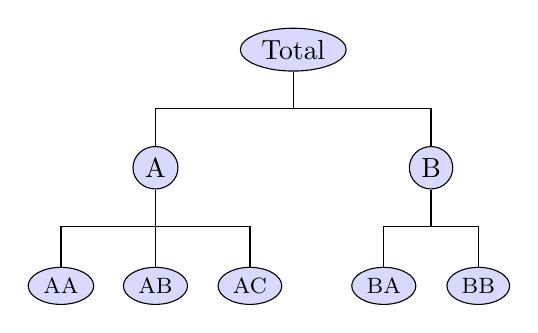
\begin{tikzpicture}
\tikzstyle{every node}=[ellipse,draw,fill=blue!15,inner sep=2pt]
\tikzstyle{level 1}=[sibling distance=3.5cm]
\tikzstyle{level 2}=[sibling distance=12mm,font=\footnotesize]
\node{Total}[edge from parent fork down]
 child {node {A}
    child {node {AA}}
    child {node {AB}}
    child {node {AC}}
    }
 child {node {B}
    child {node {BA}}
    child {node {BB}}
    %child {node {BC}}
    };
\end{tikzpicture}
\end{center}


\bibliography{sample}

\end{document} 

Hello. Nothing down here will get included.


